
%%%%%%%%%%%%%%%%%%%%%%%%%%%%%%%%%%%%%%%%%%%%%%%%%%%%%%%%%%%%%%%%%%%%%%%%
\chapter{Probability and Statistics Analysis}
%%%%%%%%%%%%%%%%%%%%%%%%%%%%%%%%%%%%%%%%%%%%%%%%%%%%%%%%%%%%%%%%%%%%%%%%

%%%%%%%%%%%%%%%%%%%%%%%%%%%%%%%%%%%%%%%%%%%%%%%%%%%%%%%%%%%%%%%%%%%%%%%%
\section{Introduction to Probability and Statistical Analysis}
%%%%%%%%%%%%%%%%%%%%%%%%%%%%%%%%%%%%%%%%%%%%%%%%%%%%%%%%%%%%%%%%%%%%%%%% this may not be the best name?

 A broadband analysis of the ambient sound level (ANL) recorded by the SHRUS was performed using the data from SHRU5. To keep consistency with the original analysis \footcite[author]{Bonnel2021}, the data for this analysis comes from SHRU5, as it had the least self noise compared to other SHRUS. Each frequency band is 50 Hz wide and centered on frequencies from 50 to 1900, 50 Hz apart, for a total of 39 frequency bands. The range was chosen as the original sampling rate ($f_{s}$) of the SHRUs is  3906.2 Hz; by the Nyquist sampling frequency, the maximum reliable frequency that can be analysed is 1951. While including a high frequency of 1950 was possible, it was omitted as being too close to the frequency limit seemed to affect the quality of the data.

Though each frequency has some independent qualities, they appear to be quantitatively linked when analyzed using a myriad of different statistics. These statistic quantities ranged from single metrics to comparing probabilities of the entire acoustic environment. While the original paper examined a frequency band around 300 Hz of 250-350 Hz, it can be assumed that this was not the only frequency propagating through the water. As this analysis would suggest, the frequency range of ambient noise under ice is broad in nature, influenced by environmental drivers such as shifting ice [CITE]. 




%%%%%%%%%%%%%%%%%%%%%%%%%%%%%%%%%%%%%%%%%%%%%%%%%%%%%%%%%%%%%%%%%%%%%%%%
\section{Probability and Statistical Analysis Methods and Results}
%%%%%%%%%%%%%%%%%%%%%%%%%%%%%%%%%%%%%%%%%%%%%%%%%%%%%%%%%%%%%%%%%%%%%%%%

\subsection{The Ambient Noise Histogram}
One of the simplest ways to visualize the differences between the three environmental conditions is by partitioning the ANL power spectral density (PSD) into histograms. After computing the sound pressure level (SPL) ANL, The bin size for each histogram was vector of 50 values, ranging from the minimum ANL to the maximum ANL of the frequency through all environmental conditions. The average bin size was around 1 Hz, with the highest frequencies having a slightly smaller bin size due to their more limited range. 

Histograms were created using the probability density function (PDF) rather than counts to show the normalized likelihood of this ANL occurring. As the acoustic data is finite, an exact PDF is not possible, leading to an estimate function. The equation for this estimate is

\begin{equation} \label{eq:finitetotvar}
\nu _{i}=\frac{c_{i}}{N \cdot w_{i}} 
\end{equation}

where $i$ refers to the bin, $\nu _{i}$ is the value of the bin, $c_{i}$ is the number of elements in the bin, and \textit{N} is the number of elements in the input data. The sum of all $\nu_{1}$, the bar size, is equivalent or almost equivalent to 1. Therefore, these histograms give the relative probability or makeup of a specific frequency's ANL in dB referenced to  $1 \mu Pa/Hz$ under the three acoustic environment conditions. From this, both the range of ambient noise and the most predominant levels are apparent. To demonstrate the conventions of an interpreting an ANL histogram, looking at a few significant figures showing the differences in acoustic environment levels is more pragmatic than examining 39 separate figures.

%%%%%%%%%%%%%%%%%%%%%%%%%%%%%%%%%%%%%%%%%%%%%%%%%%%%%%%%%%%%%%%%%%%%%%%%%
\subsubsection{Singular Frequency Histogram}
Figure \ref{fig_hist500} is an example of one histogram ranging from 450-550 Hz of the ANL for the three environmental conditions: 'ice with duct',  'ice without duct' and 'no ice'. The y-axis is the normalized count of the histogram bin, essentially operating as a percentile value. The x-axis is the ambient noise level (ANL) in dB referenced to  $1 \mu Pa/Hz$. The blue histogram is 'ice with duct', the red histogram is 'ice without duct', and the yellow histogram is 'no ice.' The environmental condition of 'no ice' also means that there is no duct. This coloring convention by acoustic environment holds for all statistic figures in this section. The number in the bins is less significant than the distribution of the histograms. 

Similar to the original paper's histogram centered at 300 Hz \footcite[author]{Bonnel2021}, this example (\autoref{fig_hist500}) has three distinct peaks for each unique acoustic environment, displaying a key effect on underwater acoustics from changes to the Arctic environment.  It would appear that the quietest ambient levels occur under the 'ice without duct' condition with a highest occurring ANL of about 64 dB. The highest levels of ambient noise belongs to  the 'no ice' condition, with the most common level being around 87 dB. The levels for 'ice with duct' are between 'ice without duct' and 'no ice', with the most common level around 72 dB. 

In terms of shape, the 'no ice' condition histogram is the most normal or Gaussian in form and also has the shortest range from approximately 74-100 dB. 'Ice with duct' seems to have a normal shape, with some right skew and 'ice without duct' is skewed heavily to the right. The two ice conditions has similar ranges from about 62-95 dB, with a matching minimum dB value likely relating the mimimum dB detectable by the SHRUs at this frequency. This minimum detection threshold does change with frequency. [cite] %(note that this floor changes with Hz) 

It is commonly said that it is quieter under ice [cite?], and this figure directly reflects that through the distribution of sound levels in these three different bins. However, this histogram shows that the presence of the Beaufort duct [cite] increases the presence of louder ambient noise at this particular bandwidth of 500 Hz. When the duct is present, the ANL is likely to be 10m dB higher than an acoustic environment without the duct. Though the range of the two 'ice' conditions is similar,  their distributions are markedly different. Metrics such as mean ANL and pairwise difference also reflect the differences between these sound metrics, but this strong difference is only present for a select range of frequencies. 

% YOU NEED TO FIX THIS IMAGE, IT STILL SAYS 300 ON IT

\begin{figure}[H]
\centering
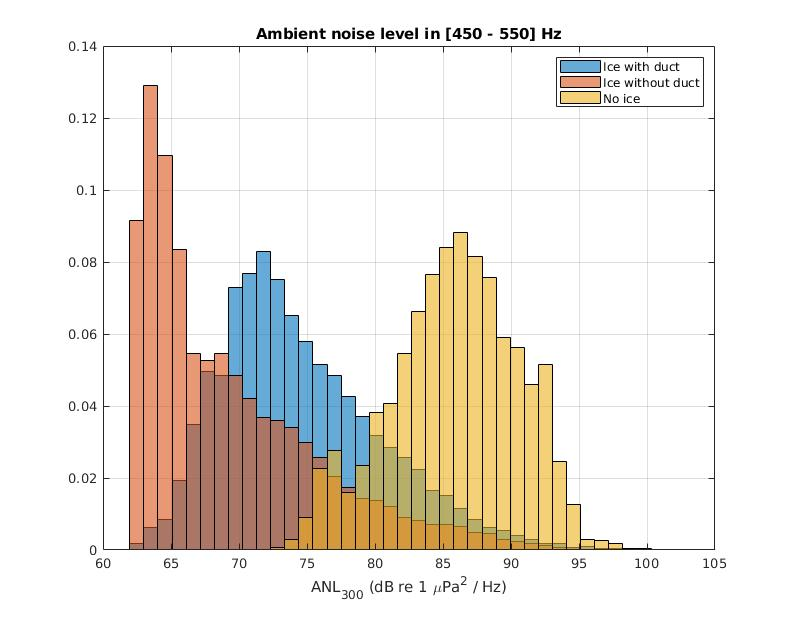
\includegraphics[scale=0.5]{Figures/ambient_hist_450_550.jpg}
\caption{Histogram of normalized ANL at 500 Hz band for conditions Ice with duct (blue) }
\label{fig_hist500}
\end{figure}

%%%%%%%%%%%%%%%%%%%%%%%%%%%%%%%%%%%%%%%%%%%%%%%%%%%%%%%%%%%%%%%%%%%%%%%%%% order above?
\subsubsection{Multiple Frequncy Ambient Noise Histogram Comparison}
Interpreting one For this section, four histograms at frequencies two mid mid high will be compared so we can see what happens
match all the axes

\textbf{Description}
This phenomena of three separate peaks is only visible from approximately 100 to 700 Hz, suggesting that these frequencies are the least likely to be trapped within the sound channel. The largest stratification between the three bins are between the frequencies of 150 Hz to 500 Hz. Ice without duct (red) is normal from 50 to about 250 Hz, after which is becomes skewed right as well. 'Ice with duct' (blue) in normal in shape from 50 to about 550 Hz, above 600 Hz is begins to be skewed right.

\textbf{Analysis}
talk about how related






\textbf{What does this mean}

\begin{figure}[H]
\centering
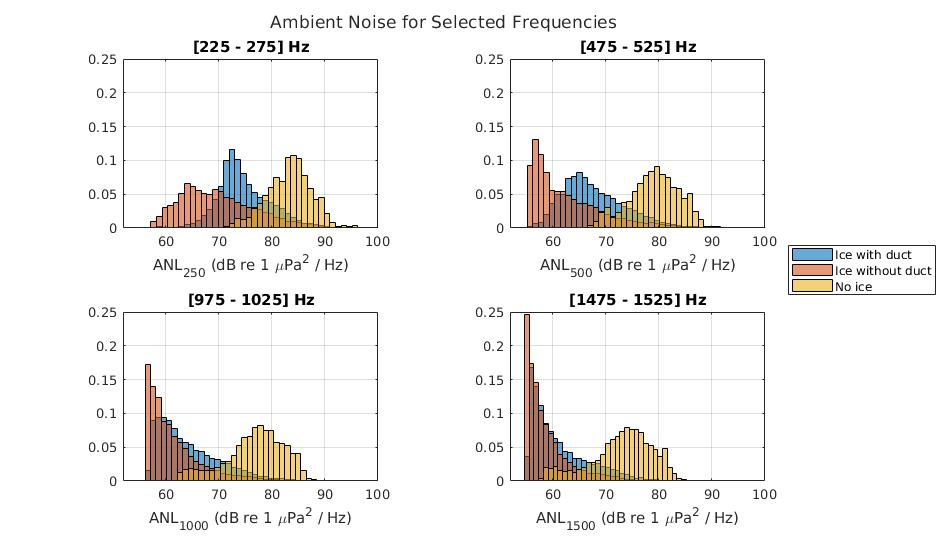
\includegraphics[scale=0.5]{Figures/selected_hists.jpg}
\caption{Histograms of ANL for 250 Hz, 500 Hz, 1000 Hz, and 1500 Hz with df normalization}
\label{fig_selhist}
\end{figure}

%%%%%%%%%%%%%%%%%%%%%%%%%%%%%%%%%%%%%%%%%%%%%%%%%%%%%%%%%%%%%%%%%%%%%%%%%
\subsection{Average ANL}
\textbf{Description}
This Figure shows the average ambient noise level generated using the mean function of MATLAB. ANL in dB referenced to $ 1 \mu Pa^{2}/Hz$ are the units of the y axis and frequency is on the x axis. The averages for ice with duct are in blue, the averages for 'ice without duct' are in red, and the 'no ice' is in yellow.

\textbf{Analysis}
The general negative trend is present across all three types, with no ice behaving linearly and ice with/without duct behaving more exponentially
In this band, and with these environmental conditions, as frequency increases, ANL decreases. Beyond 1900, the SHRUs were above the Nyquist frequency necessary to record samples so that data isn’t valid. 
There are little spikes every four points or so in the data, probably caused by the n-50 band being slightly more active at that point.

\textbf{What does this Mean}
What’s really important, and what we want to take away from this Figure 2 is WHY the ANL decreases with frequency. It’s probably because most of the ambient noise in the Arctic when there is ice is generated by the movement of the ice itself - grinding, slipping, and shearing. When there is no ice, then there is shipping, which has lots of ambient propeller noise
Things to consider: what else functions in these bandwidths of activity, like whales and other biologic factors? Is what we do going to negatively impact them?


\begin{figure}[H]
\centering
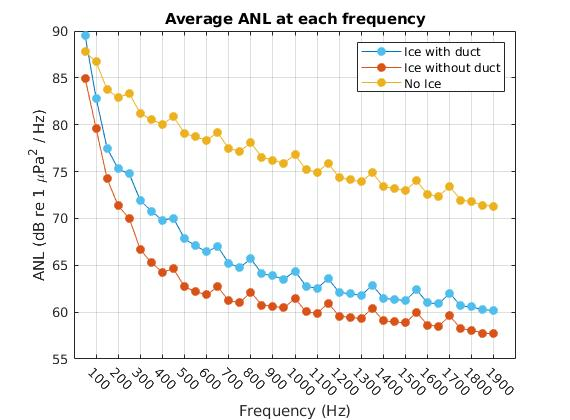
\includegraphics[scale=0.5]{Figures/Average_ANL_cutoff.jpg}
\caption{Average ANL at frequencies from 50 to 1900 Hz.}
\label{fig_avg_anl}
\end{figure}

%%%%%%%%%%%%%%%%%%%%%%%%%%%%%%%%%%%%%%%%%%%%%%%%%%%%%%%%%%%%%%%%%%%%%%%%%%%%%%%%%%%
\subsection{Total Variation Distance}
\textbf{Description}
Total variation distance is a distance in probability theory and is the absolute area between two curves. The equation is 

% equation for infinite
\begin{equation} \label{totalvardist}
\delta(,Q)=sup_{A\epsilon F}\mid P(A)-Q(A)\mid   
\end{equation}

where P and Q are probability measures on a sigma-algebra F of subsets of the sample space omega, Ω. The sigma algebra (σ-algebra/σ-filed) of a larger set A is a collection of subsets called F. For a finite data set such as this, the total variation distance is related to the L1 norm (the 1st norm for a finite dimension vector space) by the following identity:

% equation for finite
\begin{equation} \label{eq:finitetotvar}
\delta(P,Q)=\frac{1}{2}\mid P(\omega)-Q(\omega) \mid 
\end{equation}
Where $\omega$ is the finite subset of the sample space omega: $\Omega$
Total variation distance looks at all the data across all the frequencies, with the count of each bin as a proportion. It takes every value of the probability of that bin and takes the sum of the absolute difference. The range of this value for total variation distance is not constrained, and represents the “largest possible difference between the probabilities that the two probability distributions can assign to the same event,” which we can approximately translate to the largest possible difference in occurrence that a frequency can have between the two acoustic conditions. It is NOT a measure of ANL in dB but probability of occurrence between two conditions. 1 means 100\% different, 0 means 0\% different.
This data set was normalized in the function 'histcounts' using ‘Normalization’, ‘pdf’. But because its probability does that no longer become an issue
For the purposes of this analysis, the total variation distance uses the following equation: 

% equation used for our annalysis
%\begin{equation} \label{eq:actualtotvar}
%\delta(Duct, No Duct)=\frac{1}{2} \Sigma \mid Duct(f) - No Duct(f) \mid 
%\end{equation}

\begin{equation}
    \delta ^{TVD} _{ANL} ( \mathcal{A}, \mathcal{B}, \omega) = \frac{1}{2} \sum _{i} ^{} \mid \mathcal{H}_{i} [ANL^{\mathcal{A}}(\omega)-\mathcal{H}_{i} [ANL^{\mathcal{B}}(\omega)] \mid 
\end{equation}

Where N\_duct is the number in each bin of the duct condition, and N\_no\_duct is the number in each bin of the no duct condition. The integer i is equivalent to the subset of the entire set of data, and in this case refers to the specific frequency of the subset. 

\textbf{ for the new eq} where  $\cal{H}_{i}$ is the \textit{i}th bin of the environmental condition histogram $\cal{H}$, $\omega$ is the frequency band, and $\cal{A/B}$ refer to the different environmental condition being compared. $\delta$ is the total variation difference between two ANL histograms of different environmental conditions. One number is returned by this equation that sums up the total variation distance between the two conditions. The values passed to the 'histcounts' function were normalized PDF.


\textbf{Analysis}
This metric shows the probability between each data set overlapping. Since totally variation distance uses all of the data points, it only makes sense to view this frequency by frequency. The highest variation distance between the conditions ‘Ice with Duct' and 'Ice Without duct’ occurs at 50 Hz at a value of 0.44. The highest variation distance between 'ice with Duct' and 'No Ice' occurs at 600 Hz with a distance of 0.63. The highest variation distance for “no-ice and no-duct” occurs at 600 Hz and at a value of 0.72. 

\textbf{What does this Mean?}
Interpreting this graph is kind of difficult, but the easiest way to interpret it is by acoustic environment. There is a high difference between “no ice and no duct”; a mid level difference between “ice with duct and no ice”. There is the least amount of difference between “ice with duct and no duct” - the sound conditions are most similar here.
Yellow = really different conditions. Blue = more similar conditions

\begin{figure}[H]
\centering
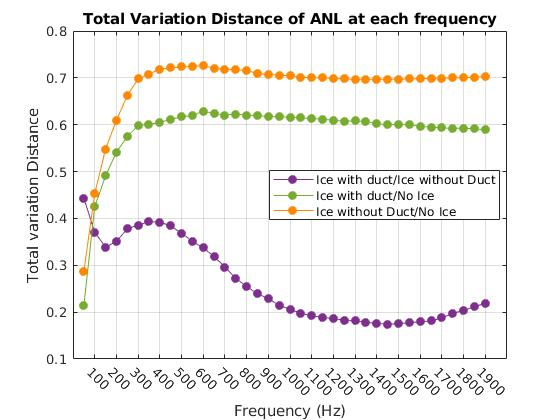
\includegraphics[scale=0.5]{Figures/recolor_total_var_dist_norm_pdf.jpg}
\caption{Total Variation distance frequencies from 50 to 1900 Hz.}
\label{fig_totvardist}
\end{figure}

%%%%%%%%%%%%%%%%%%%%%%%%%%%%%%%%%%%%%%%%%%%%%%%%%%%%%%%%%%%%%%%%%%%%%%%%%%%%%%%%
\subsection{Pairwise Difference}
\textbf{Description}
Pairwise difference is the length between the two bins at the same frequency between the two noise types being analyzed. It is different from total variation distance in that this metric is not probability but is actually the difference between the peak of each acoustic condition. Pairwise difference in the context of this analysis means the difference between each condition's histogram peaks or mode, the maximum probability occurrence of hydrophones. Because the data is being compared  is why the resulting parameter is in terms of Hz, and not a probability.
The pairwise difference was calculated using the following equation:

%pair_dist_duct_noduct(i)=edges_duct(ind_duct(i))-edges_no_duct(ind_no_duct(i))
\[Pd(f)=argmax(\cal{H}^{A}(\omega))-argmax(\cal{H}^{B}\omega)\] 	% this is not actual stat distance 
% argmax of hist-argmaxofhist, repeat equation

Where mode\_{condition} refers to the ANL bin of maximum count of that histogram, \textit{f} is the frequency of interest, and edges*. The differences are between the three conditions and are made to product positive differences (absolutes)
The xaxis of this graph is frequency in Hz, the y-axis is the difference in ANL in dB. Red denotes the difference between “no ice and ice without duct”, the yellow denotes the difference between “no ice and ice without duct” and blue denotes the difference between “ice with duct and ice without duct”

\textbf{Analysis}
The conditions with the highest overall difference are “no ice and no duct”. The condition with the lowest overall difference is “ice with duct and no duct”. The highest difference is at 450 Hz with a 23.8 db difference. The lowest difference is at 1400,1600-1800 with a difference of 0.
“No ice/ice no duct” goes up then decreases after the 450 peak; “no ice/ ice no duct” increases from 50 to 1100 Hz and mostly plateaus after. “Ice with duct and ice without duct” peaks from 200-500 then drops, going to zero in the higher frequencies

\textbf{What does this Mean?}
Similar to above, there is the least amount of difference between “Ice with duct and ice without duct.” There is the biggest difference between “ice no duct and no ice”. This means that the conditions ice with duct and ice no duct are very similar, while the conditions “ice no duct and no ice” are the most different in ANL. 
Yellow = high difference in condition - Blue = very similar condition. Peak band for all 100-900

\begin{figure}[h]
\centering
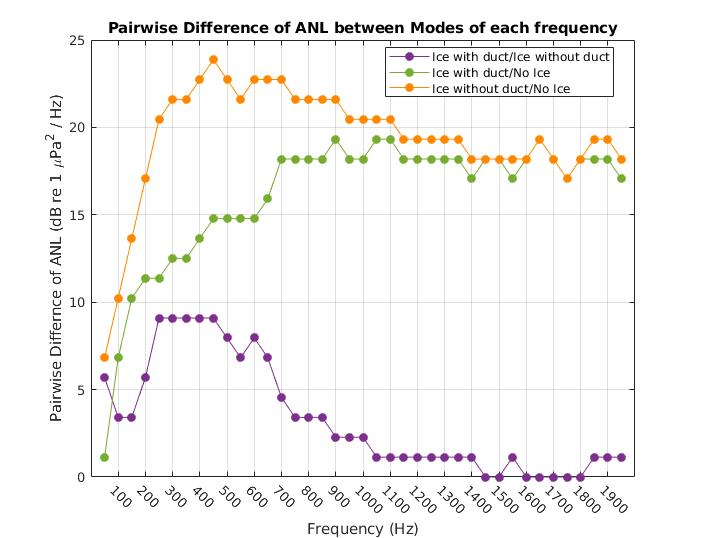
\includegraphics[scale=0.5]{Figures/recolor_pairwise_dist_ANLs.jpg}
\caption{Pairwise distance for frequencies from 50 to 1900 Hz.}
\label{fig_pairwisedist}
\end{figure}

%%%%%%%%%%%%%%%%%%%%%%%%%%%%%%%%%%%%%%%%%%%%%%%%%%%%%%%%%%%%%%%%%%%%%55
\subsection{ANL Modes}
\textbf{Description}
This is an image of the mode or most highly occurring bin of each histogram and therefore the approximate ‘most likely occurring’ sound level for that frequency

\textbf{Analysis}
There is a higher occurrence of higher dB at the lowest frequencies, which moves down thereafter
 Both the Blue Line and the red line reach down around 800 Hertz and stay low at that level.
As frequency increases, the mode of each decreases

\textbf{What does this Mean?}
Lower frequencies are louder/noisier, but as we go up in frequency Both ice with duct and eyes without duct Plateau at about 55 decibels, making this the Ambient sound noise level for these frequencies
On the other hand, it can be seen that it is significantly louder when there is no ice present in the Arctic with sound levels plateauing around 75 decibels
Louder without ice. Quieter under ice

\begin{figure}[H]
\centering
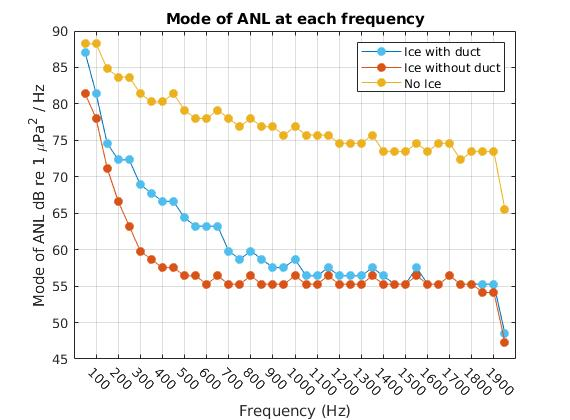
\includegraphics[scale=0.5]{Figures/mode_ANL_allfreqs.jpg}
\caption{Mode of ANL for frequencies from 50 to 1900 Hz.}
\label{fig_mode}
\end{figure}





%%%%%%%%%%%%%%%%%%%%%%%%%%%%%%%%%%%%%%%%%%%%%%%%%%%%%%%%%%%%%%%%%%%%%%%%
\subsection{Correlation Between Frequencies}
%%%%%%%%%%%%%%%%%%%%%%%%%%%%%%%%%%%%%%%%%%%%%%%%%%%%%%%%%%%%%%%%%%%%%%%%

\textbf{probs a bad way to start, fix later }Now, let's take a look at the how the frequencies are related to each other, the correlation between frequencies. In \autoref{fig_freq_corr} the correlation between each frequency is shown for each of the three environmental conditions. It is worth noting that the p-value for each of the correlations is an identity matrix, so the likely hood that the null hypothesis is true is zero percent, expect when the same frequency is compared against itself when the p-value is 1. The correlation values range from 0.4758 under the 'ice without duct' condition to 1 when frequencies are compared against themselves. 

Other than the lowest frequencies, correlation between almost all of the frequency bands is quite high. This suggests that the acoustic drivers of the Arctic's ANL are largely broadband in nature. Each environmental condition does act differently when high and low frequencies are compared to each other, resulting in different shapes of the correlation graphs. The 'no ice' condition has distinct bands of correlation around 0.7 and 0.9 for the 100-200 Hz and 200-300 Hz comparisons; elsewhere is is ~1, resulting in a boxy high correlation block. The 'ice without duct' condition  

\begin{figure}[h]
\centering
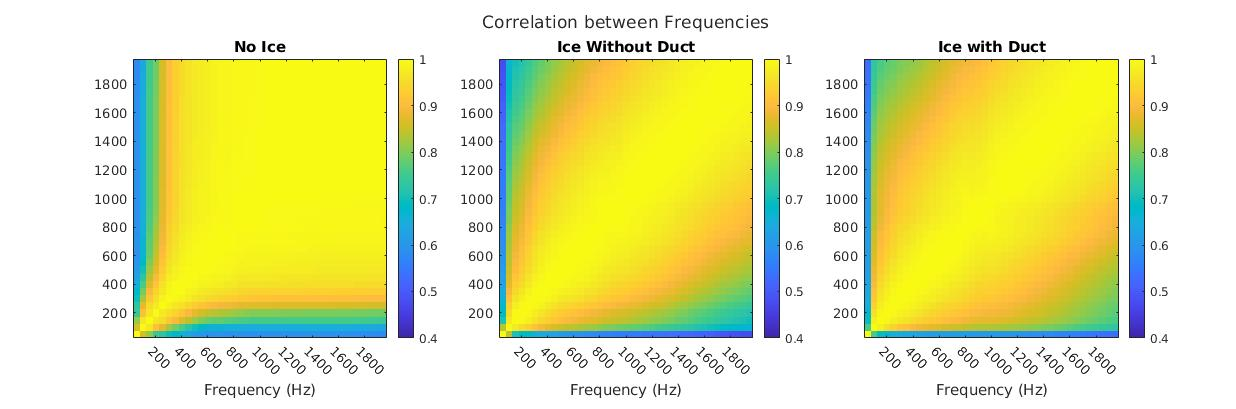
\includegraphics[scale=0.38]{Figures/corr_all_1x3.jpg}
\caption{Correlation between broadband frequencies for }
\label{fig_freq_corr}
\end{figure}




% the end of statistic section
\section{Probability and Statistics Conclusions}
% a summary of the results from above 'the what it means' section
